\documentclass[12pt,a4paper]{article}

\usepackage[a4paper,top=1in,bottom=1in,left=1in,right=1in]{geometry}
\usepackage{graphicx}
\usepackage{float}
\usepackage{amsmath}
\usepackage{newtxtext}
\usepackage{newtxmath}
\usepackage{xcolor}
\usepackage{listings}
\usepackage{caption}
\usepackage{parskip}
\usepackage[hidelinks]{hyperref}

\pagestyle{plain}
\setlength{\parindent}{0pt}
\setlength{\parskip}{0.75em}
\linespread{1.06}

\lstdefinestyle{pythoncode}{
    language=Python,
    basicstyle=\ttfamily\footnotesize,
    keywordstyle=\bfseries\color{blue!60!black},
    commentstyle=\itshape\color{green!40!black},
    stringstyle=\color{red!50!black},
    numbers=none,
    showstringspaces=false,
    breaklines=true,
    columns=fullflexible,
    keepspaces=true,
    frame=single,
    xleftmargin=1em,
    xrightmargin=0.5em,
    framexleftmargin=0.8em,
    framexrightmargin=0.5em,
    aboveskip=1em,
    belowskip=1em,
    lineskip=2pt,
    rulecolor=\color{black!35},
    backgroundcolor=\color{black!3},
    tabsize=4
}

\begin{document}

\begin{titlepage}
\thispagestyle{empty}
\centering

\vspace*{0.05in}

{\Large\bfseries TRIBHUVAN UNIVERSITY\par}
\vspace{0.16in}
{\large INSTITUTE OF ENGINEERING (IOE), PURWANCHAL CAMPUS\par}
\vspace{0.12in}
{\large DEPARTMENT OF COMPUTER AND ELECTRONICS ENGINEERING\par}

\vspace{0.45in}

\includegraphics[width=1.5in]{../assets/tu-logo.jpg}

\vspace{0.55in}
{\Large\bfseries DSAP LAB ASSIGNMENT - 2\par}

\vspace{0.3in}
{\Large\bfseries SIGNAL OPERATIONS ON BASIC SIGNALS\par}

\vspace{0.5in}
{\large\bfseries BY\par}

\vspace{0.25in}
{\large Tilak Thapa [PUR079BCT094]\par}

\vfill

{\normalsize 29 JUNE\par}

\end{titlepage}

\clearpage
\pagenumbering{arabic}
\setcounter{page}{1}

\section*{OBJECTIVE}

The objective of this lab assignment is to implement common signal operations on a basic signal generated in Lab Exercise 1 and display the results graphically. Each operation is implemented using a separate Python function.

\section*{SOFTWARE AND LIBRARIES USED}

\begin{itemize}
    \item Programming language: Python
    \item Libraries used: NumPy and Matplotlib
    \item Purpose of NumPy: numerical signal computation
    \item Purpose of Matplotlib: graphical representation of signal operations
\end{itemize}

\section*{BASE SIGNAL USED}

A rectangular signal from Lab Exercise 1 is used as the base signal. It has value 1 for a selected width and value 0 outside that interval. This signal is suitable for demonstrating amplitude scaling, time scaling, shifting, flipping, multiplication, convolution, and correlation. The original signal is shown together with the operation results in the combined output figure.

\section*{THEORY AND IMPLEMENTATION}

The following subsections describe each signal operation. The code snippets show separate Python functions used for the operations. NumPy is imported as \texttt{np} in the program.

\subsection*{1. AMPLITUDE SCALING}

Amplitude scaling changes the height or strength of a signal without changing its time position.

\[
y[n] = A x[n]
\]


Here, \(A = 2\).

\begin{lstlisting}[style=pythoncode]
# Input: signal x, scaling factor A
# Output: amplitude-scaled signal
def amplitude_scaling(x, A):
    y = A * x
    return y
\end{lstlisting}

The function returns the amplitude-scaled signal values.

\subsection*{2. TIME SCALING}

Time scaling compresses or expands a signal along the time axis.

\[
y[n] = x[an]
\]


Here, \(a = 2\).

\begin{lstlisting}[style=pythoncode]
# Input: n, signal x, scaling factor a
# Output: time-scaled signal values
def time_scaling(n, x, a):
    lookup = dict(zip(n, x, strict=True))
    y = np.array([lookup.get(a * index, 0) for index in n])
    return y
\end{lstlisting}

The function returns the time-scaled signal values.

\subsection*{3. TIME SHIFTING: TIME DELAY}

Time delay shifts a signal to the right by a selected number of samples.

\[
y[n] = x[n - k]
\]


Here, \(k = 5\).

\begin{lstlisting}[style=pythoncode]
# Input: n, signal x, delay value k
# Output: delayed signal values
def time_delay(n, x, k):
    lookup = dict(zip(n, x, strict=True))
    y = np.array([lookup.get(index - k, 0) for index in n])
    return y
\end{lstlisting}

The function returns the delayed signal values.

\subsection*{4. TIME SHIFTING: TIME ADVANCE}

Time advance shifts a signal to the left by a selected number of samples.

\[
y[n] = x[n + k]
\]


Here, \(k = 5\).

\begin{lstlisting}[style=pythoncode]
# Input: n, signal x, advance value k
# Output: advanced signal values
def time_advance(n, x, k):
    lookup = dict(zip(n, x, strict=True))
    y = np.array([lookup.get(index + k, 0) for index in n])
    return y
\end{lstlisting}

The function returns the advanced signal values.

\subsection*{5. TIME FLIPPING}

Time flipping reverses a signal around the vertical axis.

\[
y[n] = x[-n]
\]


\begin{lstlisting}[style=pythoncode]
# Input: n, signal x
# Output: time-flipped signal values
def time_flipping(n, x):
    lookup = dict(zip(n, x, strict=True))
    y = np.array([lookup.get(-index, 0) for index in n])
    return y
\end{lstlisting}

The function returns the time-flipped signal values.

\subsection*{6. MULTIPLICATION IN THE TIME DOMAIN}

Multiplication in the time domain multiplies two signals sample by sample.

\[
y[n] = x_1[n] \times x_2[n]
\]


The base rectangular signal and a delayed rectangular signal are used.

\begin{lstlisting}[style=pythoncode]
# Input: two signals x1 and x2
# Output: sample-wise multiplied signal
def time_domain_multiplication(x1, x2):
    y = x1 * x2
    return y
\end{lstlisting}

The function returns the sample-wise product of two signals.

\subsection*{7. MULTIPLICATION IN THE FREQUENCY DOMAIN}

Frequency domain multiplication is performed by multiplying the FFT values of two signals.

\[
Y[k] = X_1[k] \times X_2[k]
\]


The inverse FFT is used to show the result in the time domain.

\begin{lstlisting}[style=pythoncode]
# Input: two signals x1 and x2
# Output: inverse FFT of multiplied spectra
def frequency_domain_multiplication(x1, x2):
    X1 = np.fft.fft(x1)
    X2 = np.fft.fft(x2)
    y = np.fft.ifft(X1 * X2).real
    return y
\end{lstlisting}

The function returns the time-domain signal obtained from multiplied spectra.

\subsection*{8. CONVOLUTION}

Convolution combines two signals and is commonly used to represent the response of a system.

\[
y[n] = x[n] * h[n]
\]


The base rectangular signal and a delayed rectangular signal are used.

\begin{lstlisting}[style=pythoncode]
# Input: two signals x and h
# Output: linear convolution values
def convolution_operation(x, h):
    y = np.convolve(x, h, mode="full")
    return y
\end{lstlisting}

The function returns the linear convolution of two signals.

\subsection*{9. CORRELATION}

Correlation measures the similarity between two signals as one signal is shifted over another.

\[
r_{xy}[n] = \operatorname{corr}(x[n], y[n])
\]


The base rectangular signal and a delayed rectangular signal are used.

\begin{lstlisting}[style=pythoncode]
# Input: two signals x and y
# Output: correlation values
def correlation_operation(x, y):
    rxy = np.correlate(x, y, mode="full")
    return rxy
\end{lstlisting}

The function returns the correlation values of two signals.

\section*{OUTPUT}

The combined output image below shows the original signal and all implemented signal operation results in one view.

\begin{figure}[H]
    \centering
    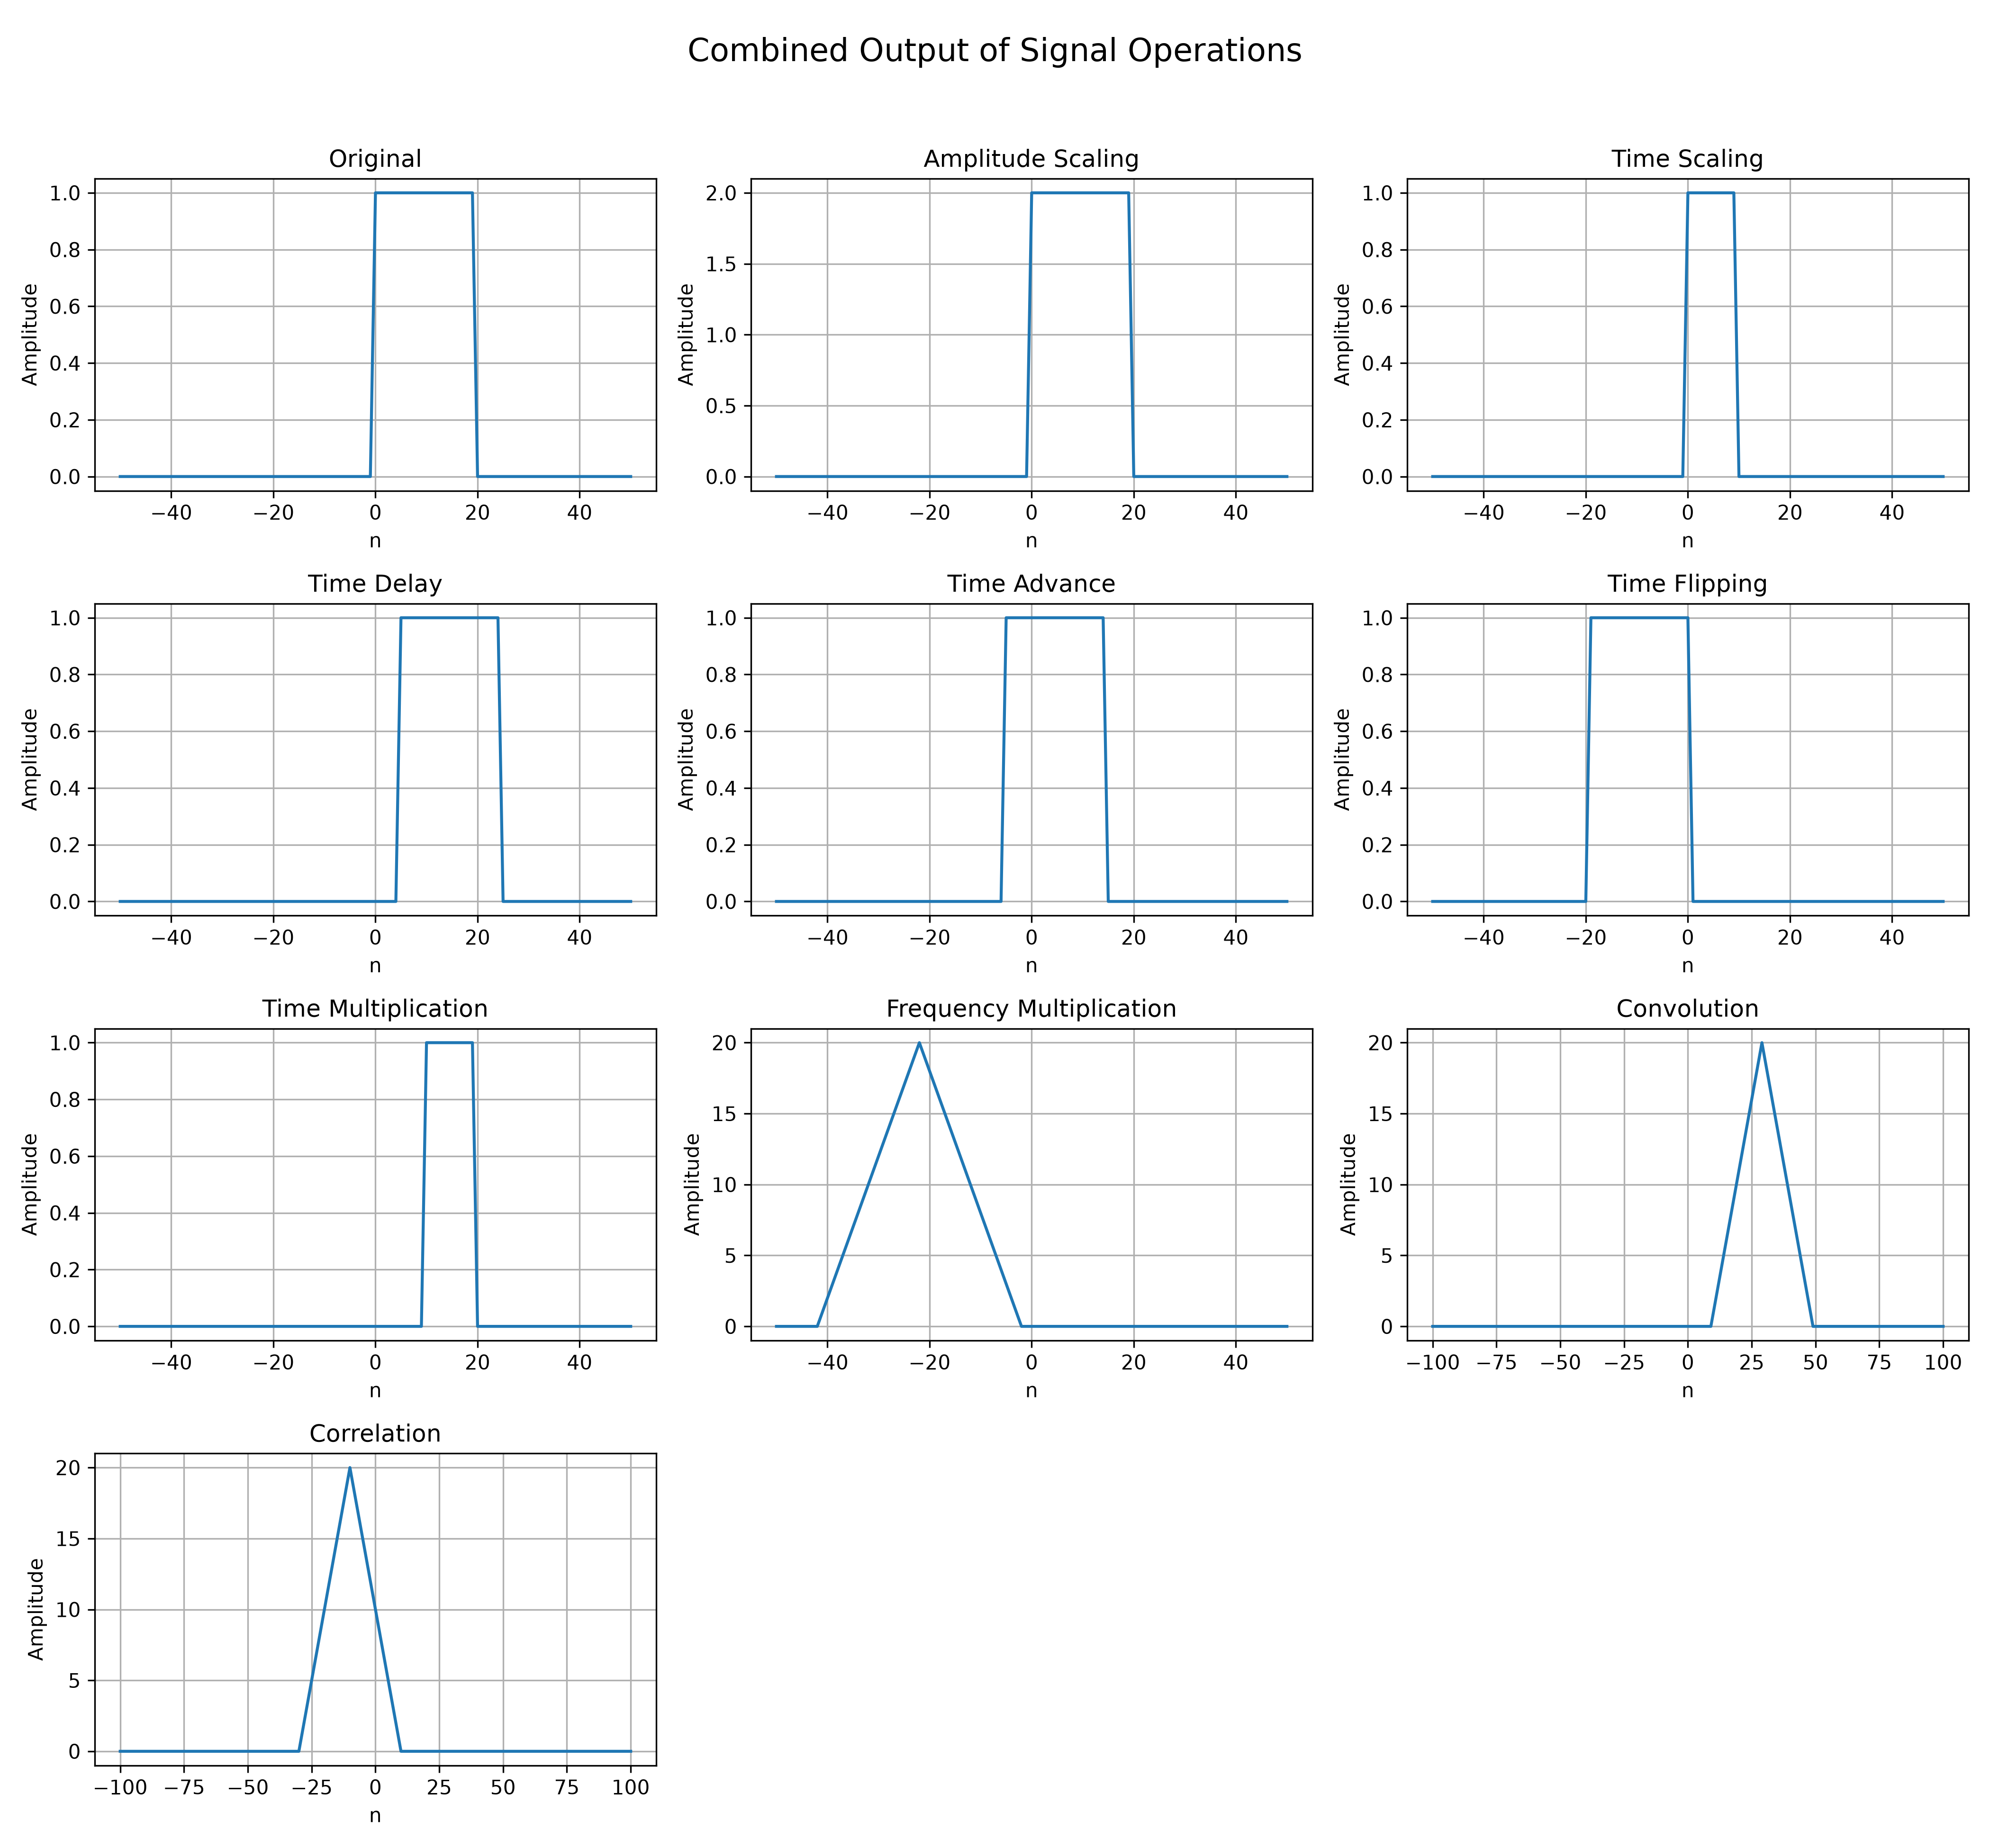
\includegraphics[width=0.92\textwidth]{combined_operations.png}
    \caption{Combined output of all implemented signal operations}
\end{figure}

\section*{RESULT AND DISCUSSION}

The output successfully demonstrates the required signal operations. Amplitude scaling changes the height of the signal. Time scaling compresses the signal along the time axis. Time delay shifts the signal to the right, while time advance shifts it to the left. Time flipping reverses the signal around the vertical axis. Multiplication in the time domain combines two signals sample by sample, and multiplication in the frequency domain combines their spectra. Convolution gives the combined response of two signals, and correlation shows the similarity between two signals.

\section*{CONCLUSION}

The lab assignment was completed by implementing each signal operation in a separate Python function and displaying the output graphically. The results show the effects of amplitude scaling, time scaling, shifting, flipping, multiplication, convolution, and correlation on a basic discrete-time signal.

\end{document}
